% Model collapse in an in-context learning transformer: the base and extended tasks.
%
% Compiles with pdfLaTeX (the Overleaf default). Every figure is drawn with
% TikZ/pgfplots from the run outputs, so no image files need uploading.
% All numbers come from the result CSVs in results/ of the repository.

\documentclass[11pt,a4paper]{article}

\usepackage[margin=2.4cm]{geometry}
\usepackage[T1]{fontenc}
\usepackage{lmodern}
\usepackage{microtype}
\usepackage{amsmath,amssymb,amsthm}
\newtheorem{proposition}{Proposition}
\usepackage{booktabs,tabularx,array}
\usepackage{xcolor}
\usepackage{tikz}
\usetikzlibrary{arrows.meta,positioning,calc}
\usepackage{pgfplots}
\pgfplotsset{compat=1.18}
\usepgfplotslibrary{groupplots}
\usepackage{caption}
\captionsetup{font=small, labelfont=bf}
\usepackage{enumitem}
\usepackage{fancyvrb}
\usepackage[hidelinks]{hyperref}

% ---------------------------------------------------------------- colours
\definecolor{modelblue}{HTML}{2A78D6}
\definecolor{realorange}{HTML}{EB6834}
\definecolor{basegreen}{HTML}{1BAF7A}
\definecolor{newgreen}{HTML}{1BAF7A}
\definecolor{badred}{HTML}{C8323D}
\definecolor{inkmuted}{HTML}{737A85}

% ---------------------------------------------------------------- notation
\newcommand{\xnext}{x_{\mathrm{next}}}
\newcommand{\ynext}{y_{\mathrm{next}}}
\newcommand{\yq}{y_{q}}
\newcommand{\data}[1]{\mathcal{D}^{(#1)}}
\newcommand{\pool}[1]{\mathcal{P}^{(#1)}}
% monospace that may break after underscores, so long file names wrap
\DeclareRobustCommand{\code}[1]{\begingroup\ttfamily\def\_{\textunderscore\allowbreak}#1\endgroup}
\newcommand{\KL}{\mathrm{KL}}

% ---------------------------------------------------------------- plot styles
\pgfplotsset{
  collapse/.style={
    width=5.25cm, height=4.6cm,
    xmin=-0.3, xmax=4.3, xtick={0,1,2,3,4},
    xlabel={Generation}, xlabel style={font=\footnotesize},
    tick label style={font=\scriptsize},
    title style={font=\footnotesize, yshift=-3pt},
    scaled y ticks=false,
    yticklabel style={/pgf/number format/fixed, /pgf/number format/precision=3},
    grid=major, grid style={draw=black!8},
    axis line style={draw=black!40},
    legend style={font=\footnotesize, draw=none, fill=none},
    legend cell align=left,
  },
  seed model/.style={modelblue!40, line width=0.5pt, forget plot},
  seed real/.style={realorange!40, line width=0.5pt, forget plot},
  seed base/.style={basegreen!40, line width=0.5pt, forget plot},
  mean model/.style={modelblue, line width=1.2pt, mark=*, mark size=1.5pt},
  mean real/.style={realorange, line width=1.2pt, mark=*, mark size=1.5pt},
  mean base/.style={basegreen, line width=1.2pt, mark=square*, mark size=1.6pt},
  ref line/.style={inkmuted, dashed, line width=0.7pt, forget plot},
}

% ---------------------------------------------------------------- diagram styles
\tikzset{
  box/.style={draw=black!45, rounded corners=3pt, align=center, font=\footnotesize,
              minimum height=1.15cm, text width=2.55cm, inner sep=3pt, fill=white},
  newbox/.style={box, draw=newgreen, line width=0.9pt, fill=newgreen!8},
  flow/.style={-{Stealth[length=2.2mm]}, draw=black!65, line width=0.6pt},
  newflow/.style={flow, draw=newgreen, dashed},
  lab/.style={font=\scriptsize, text=black!70},
}

\title{Model Collapse in an In-Context Learning Transformer\\[4pt]
\large The base and extended tasks, methodological revisions,\\
and a controlled comparison of model-generated against real data}
\author{\emph{Author names}}% replace with the group's names
\date{\today}

\begin{document}
\maketitle

\begin{abstract}
\noindent
Model collapse is the degradation of models trained on data produced by earlier
models. We study it in a setting where the true data distribution is known
exactly: a two-layer, attention-only transformer that learns a symbolic
in-context learning task. In the base task the model outputs one label, fully
determined by the context, so recursive training can only introduce errors. We
extend the task so that the model also predicts the next symbol, a uniformly
random choice between the symbols in the context, and that symbol's label. The
extended output therefore carries a real probability distribution, which
recursive training can distort.

A first five-generation run of the extended pipeline turned up four problems:
the planned collapse metric was blind to collapse by construction, the
generation-0 model memorised its training pool, generation was confounded with
the size of the training pool, and there was only one seed. We describe the
revised pipeline (per-sequence metrics computed from the model's
probabilities, checkpoint selection on held-out pool data, a matched real-data
control, and three paired seeds) and report a controlled comparison.

Because real data is never removed from the training pool, nothing runs away.
Within the model-generated chain, the KL divergence of the next-symbol
distribution from the truth moves only from 0.425 to 0.389 nats over four
recursive generations. The matched real-data control reaches 0.157 nats, so
the model-generated chain falls further behind in all three seeds, with the
gap growing every generation. Model-generated data preserves the
generation-0 model's errors, and each later model learns them as if they
were part of the task. The base pipeline, run with the same seeds, keeps its
query-label accuracy at 0.999 after four recursive generations, and
its model-written labels agree with the truth in at least 99.7\%
of sequences in every generation.
\end{abstract}

\tableofcontents
\clearpage

% =====================================================================
\section{Introduction}

Generative models are increasingly trained on data that other models
produced. Shumailov et al.~\cite{shumailov2024} showed that when each
generation of a model is trained on the previous generation's output, models
progressively lose the tails of the original distribution, a process they
called \emph{model collapse}. How quickly that happens depends on what the
training data keeps: Gerstgrasser et al.~\cite{gerstgrasser2024} found that
\emph{accumulating} synthetic data alongside the original real data, rather
than \emph{replacing} it, keeps the error bounded.

This project studies collapse in a deliberately small setting where the true
data distribution is known exactly: an attention-only transformer trained on
a symbolic in-context learning (ICL) task of the kind used to study induction
heads~\cite{olsson2022,singh2024}. Each sequence presents symbol--label pairs
whose labels are drawn afresh for every sequence, so the model can only
succeed by reading the mapping from the context.

Two pipelines are compared:
\begin{itemize}[leftmargin=1.4em]
  \item In the \textbf{base} pipeline the model predicts one token, the label
        of a queried symbol, which the context fully determines.
  \item In the \textbf{extended} pipeline the model also predicts which symbol
        comes next, a uniformly random choice between the context symbols,
        and that symbol's label. The output therefore carries a genuine
        distribution, which recursive training can distort in ways that
        accuracy does not show.
\end{itemize}

\noindent This document covers:
\begin{itemize}[leftmargin=1.4em]
  \item the tasks, model and recursive pipeline in full (Sections~\ref{sec:tasks}--\ref{sec:pipeline});
  \item how collapse is measured, including why an intuitive metric fails in
        this task (Section~\ref{sec:metrics});
  \item the four methodological problems found in the first full run, the
        evidence for each, and how the pipeline was revised
        (Section~\ref{sec:revisions});
  \item a replicated, paired comparison of model-generated against real data,
        together with the base pipeline run with the same seeds
        (Sections~\ref{sec:setup}--\ref{sec:results});
  \item what the results support and what they do not
        (Section~\ref{sec:discussion}).
\end{itemize}

% =====================================================================
\section{Background}

\subsection{In-context learning and induction heads}
An induction head is an attention circuit that, on seeing a token, looks back
to an earlier occurrence of the same token and copies whatever followed it.
Olsson et al.~\cite{olsson2022} identified such heads as a mechanism behind
in-context learning, and showed that two-layer attention-only transformers
are enough to form them. In the task used here, answering the query means
finding the context position that holds the query symbol and copying the
label that follows it, exactly the operation an induction head performs.
Singh et al.~\cite{singh2024} studied the formation of these circuits in this
kind of setup (two context pairs, five labels drawn afresh per sequence), and
the architecture below follows their defaults.

\subsection{Model collapse}
In the recursive setting, generation $i$ trains a model $M_i$ on data that
includes samples from $M_{i-1}$. Any error or bias in $M_{i-1}$ enters the
training targets of $M_i$, which may learn it as if it were real structure.
Shumailov et al.~\cite{shumailov2024} describe two compounding sources:
statistical error from finite sampling, which loses rare events first, and
functional error from the model's limited expressiveness. Gerstgrasser et
al.~\cite{gerstgrasser2024} contrast two regimes. When each generation
\emph{replaces} the previous data, the error grows with the number of
generations; when generations \emph{accumulate} on top of the original real
data, the error stays bounded. The pipeline in this project, following the
assignment, accumulates.

% =====================================================================
\section{Tasks}\label{sec:tasks}

Throughout, $N=50$ is the number of symbols, $L=5$ the number of labels and
$K=2$ the number of symbol--label pairs in the context.

\subsection{Base task}
For each sequence:
\begin{enumerate}[leftmargin=1.6em]
  \item draw $K$ distinct symbols $c_1,\dots,c_K$ uniformly without
        replacement from $\{0,\dots,N-1\}$;
  \item give each one a label $\ell(c_j)$ drawn independently and uniformly
        from $\{0,\dots,L-1\}$; the assignment is consistent within the
        sequence but drawn afresh for every sequence;
  \item draw a query index $q$ uniformly from $\{1,\dots,K\}$.
\end{enumerate}
The input is $(c_1,\ell(c_1),\dots,c_K,\ell(c_K),c_q)$, of length $2K+1=5$,
and the target is $\yq=\ell(c_q)$. Every position is a one-hot vector of
dimension $N+L=55$: symbol $c$ sets index $c$ and label $l$ sets index $N+l$.
Because labels are re-drawn every sequence, no global symbol-to-label map
exists, and the only way to answer is to read the pairing from the context.
For example, with $K=2$:
\[
  (\mathrm{A},3,\mathrm{B},1,\mathrm{A}) \mapsto 3,
  \qquad
  (\mathrm{A},0,\mathrm{C},4,\mathrm{A}) \mapsto 0 .
\]

\subsection{Extended task}
The extended task keeps the same context and query and asks for a
three-token continuation $(\yq,\xnext,\ynext)$:
\begin{itemize}[leftmargin=1.4em]
  \item $\yq=\ell(c_q)$, the query's label, exactly as in the base task;
  \item $\xnext=c_n$ with $n$ drawn uniformly from $\{1,\dots,K\}$,
        independently of $q$ (so $\xnext$ may repeat the query symbol);
  \item $\ynext=\ell(\xnext)$, the label of the chosen symbol.
\end{itemize}
The full sequence has length $2K+4=8$:
\begin{center}
\small
\begin{tabular}{l*{8}{c}}
\toprule
position & 0 & 1 & 2 & 3 & 4 & 5 & 6 & 7\\
token & $c_1$ & $\ell(c_1)$ & $c_2$ & $\ell(c_2)$ & $c_q$ & $\yq$ & $\xnext$ & $\ynext$\\
predicted from & & & & & & 4 & 5 & 6\\
\bottomrule
\end{tabular}
\end{center}
Inputs and targets share one joint vocabulary of size $V=N+L=55$, the same
layout as the one-hot inputs, so the output layer is the dual of the input
encoding.

The middle token is the point of the extension. Which symbol comes next is a
fair coin flip between the two context symbols, so the model's output at that
position should be a distribution, not a single answer. Including the query
symbol among the candidates matters: with $K=2$, excluding it would leave
exactly one candidate, $\xnext$ would be deterministic, and there would be no
distribution for recursive training to distort. The third token adds a
dependency: $\ynext$ is correct only if the model binds the symbol it just
chose to that symbol's label in the context.

\subsection{Analytic reference values}\label{sec:reference}
Because the data-generating process is fully specified, the ideal value of
every metric can be computed exactly (Table~\ref{tab:reference}).

\begin{table}[htbp]
\centering
\small
\caption{True-distribution reference values for $K=2$, $N=50$, $L=5$. The
first block is what collapse of the next-symbol choice moves; the last row is
a property of the task that no per-sequence rule can change.}
\label{tab:reference}
\begin{tabularx}{\linewidth}{Xll}
\toprule
Quantity & Value & Derivation\\
\midrule
Next-symbol choice entropy (per sequence) & $\log K = 0.693$ nats & uniform over $K$ context symbols\\
Probability on the preferred context symbol & $1/K = 0.50$ & as above\\
Probability outside the context & $0$ & $\xnext\in\{c_1,\dots,c_K\}$\\
KL from the true next-symbol distribution & $0$ & definition\\
\midrule
Cross-entropy floor at $\xnext$ & $\log K = 0.693$ nats & entropy of the true choice\\
Accuracy ceiling at $\xnext$ & $1/K = 0.50$ & any argmax hits half the time\\
Floor of the mean loss over three tokens & $\log K/3 = 0.231$ nats & $(0+\log K+0)/3$\\
\midrule
Chance accuracy for $\yq$, $\ynext$ & $1/L = 0.20$ & uniform guess\\
Accuracy without binding & $1/K+(1-1/K)/L = 0.60$ & see text\\
\midrule
Entropy of the emitted-symbol marginal & $\log N = 3.912$ nats & Proposition~\ref{prop:marginal}\\
\bottomrule
\end{tabularx}
\end{table}

\paragraph{The no-binding baseline.} A model that has learned ``the answer is
one of the context labels'' but not which label belongs to which symbol can
copy a context label at random. It is right when it copies the correct pair
(probability $1/K$), and otherwise right by luck when the other pair happens to
carry the same label (probability $1/L$). Its accuracy is
\[
  \frac{1}{K}+\Bigl(1-\frac{1}{K}\Bigr)\frac{1}{L}=\frac12+\frac12\cdot\frac15=0.60 .
\]
Accuracy above $0.60$, not above $0.20$, is therefore the evidence that the
model performs in-context binding.

% =====================================================================
\section{Model}\label{sec:model}

\subsection{Architecture}
Both pipelines use the same causal, attention-only transformer, following the
defaults of Singh et al.~\cite{singh2024}: two layers, eight heads, model
width $d=64$ (head width 8), rotary position embeddings
(RoPE~\cite{su2021}) on queries and keys, pre-layer normalisation, residual
connections and no MLP blocks. With $e_t\in\{0,1\}^{55}$ the one-hot input at
position $t$:
\begin{align}
  h^{(0)}_t &= W_{\mathrm{in}}\, e_t + b_{\mathrm{in}},\\
  h^{(l)} &= h^{(l-1)} + \mathrm{MHA}_l\!\bigl(\mathrm{LN}_l(h^{(l-1)})\bigr),\qquad l=1,2,\\
  z_t &= W_{\mathrm{out}}\,\mathrm{LN}\bigl(h^{(2)}_t\bigr) + b_{\mathrm{out}},
\end{align}
where $\mathrm{MHA}_l$ is causal multi-head self-attention with a bias-free
joint query--key--value projection and a bias-free output projection. The
extended model imports the base model's blocks rather than copying them, so
the two architectures are identical by construction. They differ only in the
readout (Table~\ref{tab:params}):
\begin{itemize}[leftmargin=1.4em]
  \item \textbf{base:} $W_{\mathrm{out}}\in\mathbb{R}^{5\times 64}$, read at the
        query position $2K$;
  \item \textbf{extended:} $W_{\mathrm{out}}\in\mathbb{R}^{55\times 64}$, read at
        positions $2K$, $2K+1$ and $2K+2$, each predicting the token that
        follows it. The logits are deliberately not restricted by token type,
        so emitting a symbol where a label belongs (or the reverse) is a
        real, measurable error.
\end{itemize}

\begin{table}[htbp]
\centering
\small
\caption{Parameter counts.}
\label{tab:params}
\begin{tabular}{lrr}
\toprule
Component & Base & Extended\\
\midrule
Input projection ($55\to 64$, with bias) & 3{,}584 & 3{,}584\\
Two attention blocks (each: LayerNorm 128, QKV 12{,}288, output 4{,}096) & 33{,}024 & 33{,}024\\
Final LayerNorm & 128 & 128\\
Output head & 325 & 3{,}575\\
\midrule
Total & 37{,}061 & 40{,}311\\
\bottomrule
\end{tabular}
\end{table}

\subsection{Training objective}
Both models are trained with Adam~\cite{kingma2015} at learning rate $10^{-4}$,
batch size 32 (sampled with replacement from the training pool) for 20{,}000
steps. The base model minimises the cross-entropy of $\yq$. The extended model
is trained with teacher forcing: the true continuation sits in the input, all
three positions are predicted in one forward pass, and the loss is the mean of
the three per-token cross-entropies. The three per-token losses are also
logged separately, because the mean is dominated by the irreducible $\log K$
term at $\xnext$.

\subsection{Generating continuations}
When a trained model writes training data for the next generation:
\begin{itemize}[leftmargin=1.4em]
  \item the \textbf{base} model's prediction is the argmax label, which is
        appropriate because its target is deterministic;
  \item the \textbf{extended} model generates autoregressively in three
        forward passes. At each step it reads the logits at the current
        position, chooses a token and writes that token's one-hot vector into
        the next input position before predicting the following token.
\end{itemize}
The rollout has to be autoregressive because $\ynext$ must be conditioned on
the symbol the model actually emitted. Three decoding rules are available:
\code{sample} (multinomial at temperature 1, used for every result here),
\code{argmax}, and \code{hybrid} (argmax for $\yq$ and $\ynext$, sampling for
$\xnext$). Argmax would make the model always emit its favourite of the two
context symbols, removing the coin flip from the data in a single generation.

% =====================================================================
\section{Recursive training pipeline}\label{sec:pipeline}

\begin{enumerate}[leftmargin=1.6em]
  \item \textbf{Fixed evaluation sets.} A validation set and a test set of
        2{,}000 sequences each are drawn once from the true distribution and
        reused, unchanged, in every generation.
  \item \textbf{Generation 0.} $\data{0}$ holds 5{,}000 sequences from the true
        distribution, with true targets.
  \item \textbf{Generation $i\ge 1$.} 5{,}000 fresh contexts are drawn from the
        true distribution, and their targets (base) or continuations (extended)
        are written by $M_{i-1}$. Contexts are always real, so the only way
        model error enters is through the generated tokens.
  \item \textbf{Accumulation.} Model $M_i$ trains on the pool
        $\pool{i}=\data{0}\cup\dots\cup\data{i}$ of $5{,}000\,(i+1)$ sequences.
        Real data is never removed.
  \item \textbf{Fresh start.} Every $M_i$ is initialised from scratch, never
        warm-started from $M_{i-1}$.
\end{enumerate}

\begin{figure}[htbp]
\centering
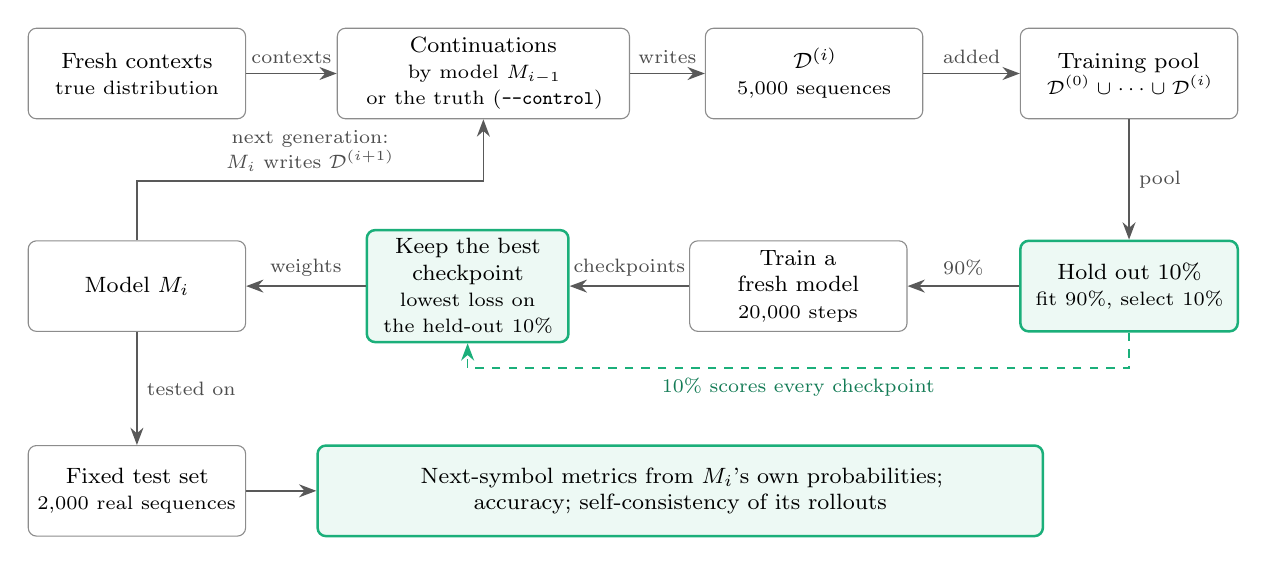
\begin{tikzpicture}
  \node[box] (ctx) at (0,0) {Fresh contexts\\{\scriptsize true distribution}};
  \node[box, text width=3.5cm] (src) at (4.4,0)
       {Continuations\\{\scriptsize by model $M_{i-1}$}\\{\scriptsize or the truth (\code{-{}-control})}};
  \node[box] (dat) at (8.6,0) {$\data{i}$\\{\scriptsize 5{,}000 sequences}};
  \node[box] (pool) at (12.6,0) {Training pool\\{\scriptsize $\data{0}\cup\dots\cup\data{i}$}};

  \node[newbox] (split) at (12.6,-2.7) {Hold out 10\%\\{\scriptsize fit 90\%, select 10\%}};
  \node[box] (train) at (8.4,-2.7) {Train a fresh model\\{\scriptsize 20{,}000 steps}};
  \node[newbox, text width=2.35cm] (keep) at (4.2,-2.7) {Keep the best checkpoint\\{\scriptsize lowest loss on}\\{\scriptsize the held-out 10\%}};
  \node[box] (model) at (0,-2.7) {Model $M_i$};

  \node[box] (test) at (0,-5.3) {Fixed test set\\{\scriptsize 2{,}000 real sequences}};
  \node[newbox, text width=9.0cm] (metrics) at (6.9,-5.3)
       {Next-symbol metrics from $M_i$'s own probabilities;\\
        accuracy; self-consistency of its rollouts};

  \draw[flow] (ctx) -- node[lab, above] {contexts} (src);
  \draw[flow] (src) -- node[lab, above] {writes} (dat);
  \draw[flow] (dat) -- node[lab, above] {added} (pool);
  \draw[flow] (pool) -- node[lab, right] {pool} (split);
  \draw[flow] (split) -- node[lab, above] {90\%} (train);
  \draw[flow] (train) -- node[lab, above] {checkpoints} (keep);
  \draw[flow] (keep) -- node[lab, above] {weights} (model);
  \draw[newflow] (split.south) -- ++(0,-0.45) -| node[lab, pos=0.25, below, text=newgreen!70!black] {10\% scores every checkpoint} (keep.south);
  \draw[flow] (model.north) -- ++(0,0.75) -| node[lab, pos=0.25, above, align=center] {next generation:\\$M_i$ writes $\data{i+1}$} (src.south);
  \draw[flow] (model) -- node[lab, right] {tested on} (test);
  \draw[flow] (test) -- (metrics);
\end{tikzpicture}
\caption{One generation of the extended pipeline. Green boxes are the
revisions of Section~\ref{sec:revisions}. The base pipeline has the same loop
with a single argmax target, no held-out selection and no control.}
\label{fig:pipeline}
\end{figure}

Table~\ref{tab:pipelines} summarises how the two pipelines differ as run for
this report.

\begin{table}[htbp]
\centering
\small
\caption{Base and extended pipelines as run for this report. Task,
architecture and optimiser settings are identical.}
\label{tab:pipelines}
\begin{tabularx}{\linewidth}{lXX}
\toprule
 & Base & Extended\\
\midrule
Tokens generated per sequence & 1 ($\yq$) & 3 ($\yq$, $\xnext$, $\ynext$)\\
How generated tokens are chosen & argmax & sampled at temperature 1\\
Checkpoint kept each generation & last step & lowest loss on a held-out 10\% of the pool\\
Control condition & none & matched real-data control\\
Seeds & 1, 2, 3 & 1, 2, 3 in each condition\\
Collapse measures & test accuracy and loss; agreement of generated labels with the truth & per-token accuracy and loss; per-sequence next-symbol metrics; self-consistency; generated-data statistics\\
Script & \code{src/train\_collapse.py} & \code{src/train\_extended\_collapse.py}\\
\bottomrule
\end{tabularx}
\end{table}

% =====================================================================
\section{Measuring collapse}\label{sec:metrics}

All model metrics are measured on the fixed test set, so a change across
generations reflects the model, not a new sample of contexts.

\subsection{Accuracy and loss per token}
Per-token cross-entropy and argmax accuracy are computed with teacher forcing
on the test set. Accuracy on $\yq$ and $\ynext$ measures correctness; accuracy
on $\xnext$ is capped at $1/K$ by construction and carries little
information.

\subsection{The next-symbol distribution}\label{sec:nextsym}
For test sequence $n$, let $C_n=\{c_{n,1},\dots,c_{n,K}\}$ be its context
symbols and $p_n(\cdot)$ the model's softmax distribution at the $\xnext$
slot (conditioned on the true $\yq$). Define the in-context mass and the
renormalised choice
\[
  m_n=\sum_{j=1}^{K}p_n(c_{n,j}),\qquad
  \tilde p_{n,j}=\frac{p_n(c_{n,j})}{m_n}.
\]
The four next-symbol metrics, each averaged over the $T=2{,}000$ test
sequences, are
\begin{align}
  \text{choice entropy}\quad &\bar H=\frac1T\sum_{n}\Bigl(-\sum_{j}\tilde p_{n,j}\log\tilde p_{n,j}\Bigr), \\
  \text{preferred-symbol probability}\quad &\bar\pi=\frac1T\sum_{n}\max_j\tilde p_{n,j}, \\
  \text{off-context probability}\quad &\bar o=\frac1T\sum_{n}\bigl(1-m_n\bigr), \\
  \text{KL from truth}\quad &\overline{\KL}=\frac1T\sum_{n}\KL\bigl(u_n\,\|\,p_n\bigr)
     =\frac1T\sum_{n}\Bigl(-\log K-\frac1K\sum_{j}\log p_n(c_{n,j})\Bigr),
\end{align}
where $u_n$ is the true distribution, uniform on $C_n$. The choice entropy and
preferred-symbol probability measure how decisively the model commits to one
context symbol; the renormalisation stops leakage from inflating them. The
off-context probability measures leakage to anything that was never in the
context, wrong symbols and wrong-type tokens alike. The KL combines both
failure modes; it equals the expected $\xnext$ test loss minus $\log K$, but is
computed exactly instead of from one sampled target per sequence. Each metric
was checked against hand-built distributions with known answers before use
(uniform, deterministic, leaking and biased).

These quantities must be computed from probabilities. A generated dataset
holds one sampled $\xnext$ per context, so no statistic of the data alone can
show how sure the model was when it chose.

\subsection{Self-consistency and type validity}
The trained model generates continuations for the fixed test contexts. Among
the sequences whose emitted $\hat x_n$ is a context symbol, self-consistency is
the share whose emitted $\hat y_n$ equals that symbol's label in the context.
It asks whether the model still binds symbol to label on its \emph{own}
generated symbol. A model whose choice has collapsed onto a favourite can
still be perfectly self-consistent, whereas one whose binding has degraded
cannot. It is a behavioural measure: attributing it to a specific circuit
would require attention analysis or ablations. Type validity is the share of
emitted tokens of the right kind for their slot (labels at positions 5 and 7,
a symbol at position 6).

\subsection{Statistics of the generated data}
For each $\data{i}$, the pipeline records the share of sequences whose $\xnext$
lies in the context, the agreement of each generated token with the
continuation the true distribution would have produced for the same context,
and the self-consistency of the generated data. Row $i$ of these columns
describes data written by $M_{i-1}$, not by $M_i$.

\subsection{Why the emitted-symbol histogram cannot detect collapse}\label{sec:blind}
The original design measured collapse through the histogram of emitted
$\xnext$ symbols over all $N$ symbols: its entropy, coverage and top-1 mass.
In this task that histogram cannot see per-sequence collapse.

\begin{proposition}\label{prop:marginal}
Let the context symbols be drawn uniformly without replacement, and let a rule
choose $\xnext=c_{\sigma}$, where the slot $\sigma\in\{1,\dots,K\}$ may depend
on the slot structure of the sequence (for example the query index) but not
on which symbols occupy the slots. Then $\Pr(\xnext=s)=1/N$ for every symbol
$s$, whatever the rule.
\end{proposition}

\noindent\emph{Proof.} By exchangeability, the symbol in each slot is
marginally uniform on $\{0,\dots,N-1\}$, and this stays true conditional on
the slot structure, which is drawn independently of the symbols. Choosing a
slot without looking at the symbols therefore gives
$\Pr(\xnext=s)=\sum_k\Pr(\sigma=k)\Pr(c_k=s)=\sum_k\Pr(\sigma=k)/N=1/N$.\hfill$\square$

\smallskip
A rule that always picks the first context symbol is completely collapsed
(choice entropy 0) yet produces a perfectly uniform histogram. A rule that
looks at symbol identities, for example ``always the smaller id'', can skew
the histogram, so the histogram remains useful as a check for \emph{global}
symbol bias. Section~\ref{sec:r1} shows the effect empirically.

% =====================================================================
\section{Methodological revisions}\label{sec:revisions}

The first version of the extended pipeline ran end to end and produced clean
figures. A full five-generation run (seed 5, before any revision; per-
generation results in Table~\ref{tab:firstrun}) then turned up four problems,
each serious enough to make a conclusion unreliable.

\subsection{Why rigour matters for this project}
Every claim this project makes is a comparison: extended against base, later
generations against earlier ones, model-generated against real data. A
comparison is only as trustworthy as the instrument that measures it and the
controls around it. The first run's headline metric showed the true value,
flat, in all five generations, which reads as ``no collapse''. That flat line
turned out to be guaranteed by construction
(Proposition~\ref{prop:marginal}). Written up as it stood, the conclusion
would have been an artefact of the measurement, not a property of the model.

Synthetic tasks make rigour cheap: the true distribution is known
analytically, every part of the data-generating process is under control,
and a run takes half an hour on a laptop. The revisions therefore follow four
rules:
\begin{enumerate}[leftmargin=1.6em]
  \item \textbf{Check every metric against a known answer}, a healthy case and
        a collapsed one, before trusting what it says.
  \item \textbf{Attribute an effect to recursive training only against a
        matched control} that changes nothing else.
  \item \textbf{Replicate before interpreting}: report trends across several
        seeds, with every seed visible.
  \item \textbf{Keep the truth out of the loop}: data used to evaluate the
        models never decides what the loop trains on or which checkpoint it
        keeps.
\end{enumerate}

\subsection{Revision 1: measure collapse where it can happen}\label{sec:r1}
\paragraph{Problem.} The emitted-symbol histogram cannot detect per-sequence
collapse (Section~\ref{sec:blind}).
\paragraph{Evidence.} Hand-built choices for 5{,}000 sequences were passed
through the original metric (Table~\ref{tab:blind}, Figure~\ref{fig:hist}).
The completely collapsed rules are indistinguishable from the truth. In the
first run, the histogram stayed between 3.897 and 3.909 nats with 50/50
coverage in every generation, while the entropy of the model's own
next-symbol distribution ranged from 0.337 to 0.712 nats
(Table~\ref{tab:firstrun}). The original claim that argmax decoding would
``destroy the symbol distribution in a single generation'' was wrong for the
same reason: argmax would remove the coin flip from the data, but the
histogram would not show it.
\paragraph{Change.} Collapse is now measured from $M_i$'s probabilities on the
fixed test contexts (Section~\ref{sec:nextsym}). The histogram is kept and
relabelled as a global bias check.

\begin{table}[htbp]
\centering
\small
\caption{The emitted-symbol histogram under hand-built rules, 5{,}000
sequences. Fully collapsed rules score the same as the truth.}
\label{tab:blind}
\begin{tabular}{lccc}
\toprule
How $\xnext$ is chosen & Histogram entropy & Coverage & Choice entropy\\
\midrule
Truth: coin flip between the two context symbols & 3.908 & 50/50 & 0.693\\
Always the first context symbol & 3.907 & 50/50 & 0\\
Always repeat the query symbol & 3.907 & 50/50 & 0\\
Always the smaller symbol id & 3.712 & 49/50 & 0\\
\bottomrule
\end{tabular}
\end{table}

\begin{figure}[htbp]
\centering
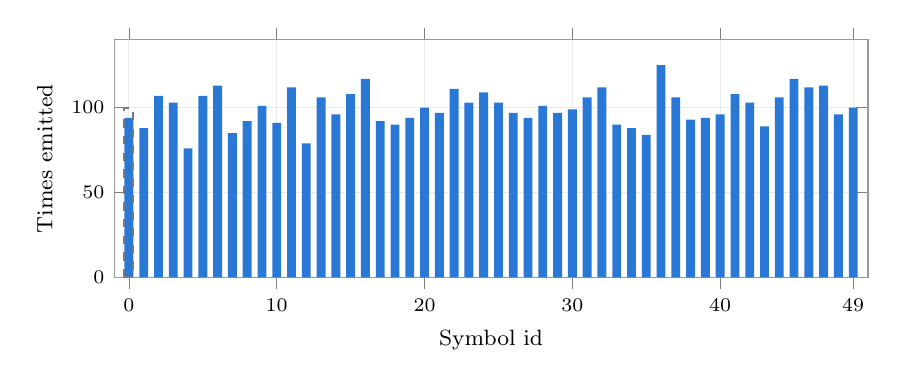
\begin{tikzpicture}
\begin{axis}[
  width=0.92\linewidth, height=4.6cm,
  ybar, bar width=3.2pt,
  xmin=-1, xmax=50, ymin=0, ymax=140,
  xlabel={Symbol id}, ylabel={Times emitted},
  xlabel style={font=\footnotesize}, ylabel style={font=\footnotesize},
  tick label style={font=\scriptsize},
  grid=major, grid style={draw=black!8}, axis line style={draw=black!40},
  xtick={0,10,20,30,40,49},
]
\addplot[fill=modelblue, draw=none] coordinates {(0,94) (1,88) (2,107) (3,103) (4,76) (5,107) (6,113) (7,85) (8,92) (9,101) (10,91) (11,112) (12,79) (13,106) (14,96) (15,108) (16,117) (17,92) (18,90) (19,94) (20,100) (21,97) (22,111) (23,103) (24,109) (25,103) (26,97) (27,94) (28,101) (29,97) (30,99) (31,106) (32,112) (33,90) (34,88) (35,84) (36,125) (37,106) (38,93) (39,94) (40,96) (41,108) (42,103) (43,89) (44,106) (45,117) (46,112) (47,113) (48,96) (49,100)};
\addplot[ref line, domain=-1:50, samples=2] {100};
\end{axis}
\end{tikzpicture}
\caption{Emitted-symbol histogram of a completely collapsed rule (always pick
the first context symbol) over 5{,}000 sequences. The dashed line is the
uniform expectation of 100 per symbol. Entropy 3.907 nats, against 3.908 for
the truth.}
\label{fig:hist}
\end{figure}

\subsection{Revision 2: stop training before the model memorises its pool}\label{sec:r2}
\paragraph{Problem.} 20{,}000 steps at batch size 32 over a 5{,}000-sequence
pool is 128 passes over the data. Trained to the last step, $M_0$ memorised
which symbol came next in each training sequence.
\paragraph{Evidence.} Figure~\ref{fig:overfit}. From step 8{,}000 onwards,
$M_0$'s training loss was below the lowest value the coin flip allows
($0.231$), reaching 0.036 at step 15{,}000. Its next-symbol loss on held-out
data bottomed out at 1.06 at step 5{,}000 and rose to 2.08 at step 20{,}000,
three times its floor. On the test set, $M_0$ put 0.878 of its probability on
its preferred context symbol (truth 0.5) and was over 90\% sure in 63\% of
sequences. It was collapsed before any recursion happened, so every later
generation would have been measured against a broken baseline.
\paragraph{Change.} 10\% of each generation's pool is held out uniformly at
random. Every 500 steps the model is evaluated on it, and the checkpoint with
the lowest held-out loss is kept (\code{select\_holdout\_fraction: 0.1}). The
selection uses the pool rather than the fixed validation set because that set
is real data. Choosing checkpoints with it would let the true distribution
steer every generation of the synthetic loop, which can only hide collapse.
The pool is all a model in the loop would have.

\begin{figure}[htbp]
\centering
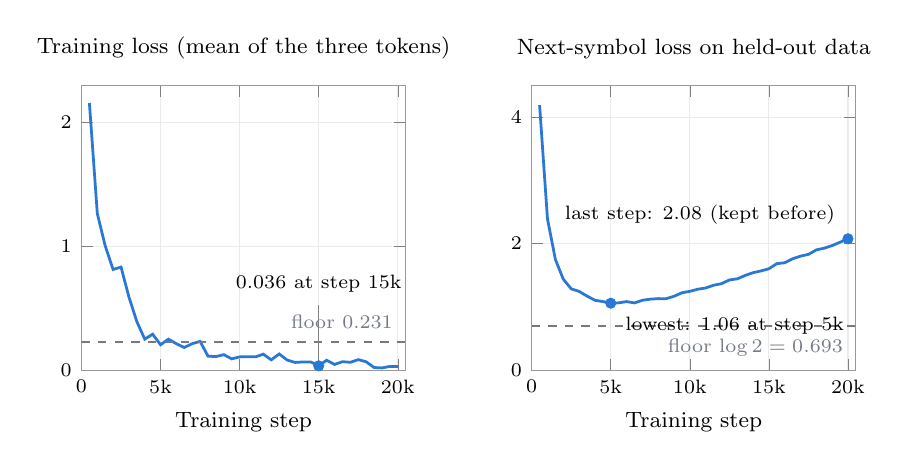
\begin{tikzpicture}
\begin{groupplot}[
  group style={group size=2 by 1, horizontal sep=1.6cm},
  width=0.47\linewidth, height=5.2cm,
  xmin=0, xmax=20500, xtick={0,5000,10000,15000,20000},
  xticklabels={0,5k,10k,15k,20k}, scaled x ticks=false,
  xlabel={Training step}, xlabel style={font=\footnotesize},
  tick label style={font=\scriptsize}, title style={font=\footnotesize},
  grid=major, grid style={draw=black!8}, axis line style={draw=black!40},
  ymin=0,
]
\nextgroupplot[title={Training loss (mean of the three tokens)}, ymax=2.3]
\addplot[modelblue, line width=1pt] coordinates {(500,2.1579) (1000,1.2652) (1500,1.0036) (2000,0.8140) (2500,0.8335) (3000,0.5915) (3500,0.3933) (4000,0.2516) (4500,0.2917) (5000,0.2065) (5500,0.2520) (6000,0.2146) (6500,0.1844) (7000,0.2151) (7500,0.2335) (8000,0.1140) (8500,0.1113) (9000,0.1265) (9500,0.0925) (10000,0.1086) (10500,0.1095) (11000,0.1089) (11500,0.1305) (12000,0.0846) (12500,0.1320) (13000,0.0833) (13500,0.0638) (14000,0.0675) (14500,0.0675) (15000,0.0363) (15500,0.0815) (16000,0.0474) (16500,0.0696) (17000,0.0650) (17500,0.0863) (18000,0.0689) (18500,0.0227) (19000,0.0194) (19500,0.0317) (20000,0.0313)};
\addplot[ref line, domain=0:20500, samples=2] {0.231};
\node[font=\scriptsize, text=inkmuted, anchor=south east] at (axis cs:20300,0.26) {floor 0.231};
\addplot[only marks, mark=*, mark size=1.8pt, modelblue] coordinates {(15000,0.0363)};
\node[font=\scriptsize, anchor=south] at (axis cs:15000,0.55) {0.036 at step 15k};
\draw[black!50] (axis cs:15000,0.07) -- (axis cs:15000,0.53);
\nextgroupplot[title={Next-symbol loss on held-out data}, ymax=4.5]
\addplot[modelblue, line width=1pt] coordinates {(500,4.1885) (1000,2.3907) (1500,1.7502) (2000,1.4387) (2500,1.2874) (3000,1.2467) (3500,1.1725) (4000,1.1064) (4500,1.0860) (5000,1.0602) (5500,1.0657) (6000,1.0855) (6500,1.0648) (7000,1.1068) (7500,1.1241) (8000,1.1324) (8500,1.1317) (9000,1.1693) (9500,1.2246) (10000,1.2475) (10500,1.2809) (11000,1.3002) (11500,1.3435) (12000,1.3681) (12500,1.4271) (13000,1.4448) (13500,1.4983) (14000,1.5423) (14500,1.5699) (15000,1.6042) (15500,1.6850) (16000,1.6985) (16500,1.7612) (17000,1.8034) (17500,1.8311) (18000,1.9023) (18500,1.9292) (19000,1.9703) (19500,2.0235) (20000,2.0782)};
\addplot[ref line, domain=0:20500, samples=2] {0.6931};
\node[font=\scriptsize, text=inkmuted, anchor=north east] at (axis cs:20300,0.65) {floor $\log 2 = 0.693$};
\addplot[only marks, mark=*, mark size=1.8pt, modelblue] coordinates {(5000,1.0602) (20000,2.0782)};
\node[font=\scriptsize, anchor=north west] at (axis cs:5300,1.0) {lowest: 1.06 at step 5k};
\node[font=\scriptsize, anchor=south east] at (axis cs:19800,2.15) {last step: 2.08 (kept before)};
\end{groupplot}
\end{tikzpicture}
\caption{Generation 0 of the first (pre-revision) run, seed 5. Training loss
fell below the lowest value the coin flip allows, while the next-symbol loss
on held-out data rose after step 5{,}000. The original pipeline kept the last
step; the revised one keeps the checkpoint with the lowest held-out loss.}
\label{fig:overfit}
\end{figure}

\subsection{Revision 3: a matched real-data control}\label{sec:r3}
\paragraph{Problem.} The pool grows every generation (from 5{,}000 to 25{,}000
sequences) while the training budget stays fixed, so ``later generation'' also
means ``more data, and fewer passes over it''. Any trend across generations
mixes the two.
\paragraph{Evidence.} In the first run the entropy of the model's next-symbol
distribution \emph{rose} from 0.337 to 0.712 nats across generations
(Table~\ref{tab:firstrun}), the opposite of collapse and most likely the
memorisation fading as the pool grew.
\paragraph{Change.} The \code{-{}-control} flag reruns the identical pipeline
with every generation's continuations drawn from the true distribution, so
the pool grows to the same sizes but never holds model output
(Figure~\ref{fig:pool}). It is a flag on the same configuration file rather
than a second file, so the two conditions cannot drift apart. With the same
seed both conditions draw identical $\data{0}$ and train identical $M_0$, so
each seed is a paired comparison and only the gap between the conditions is
attributed to training on model output.

\begin{figure}[htbp]
\centering
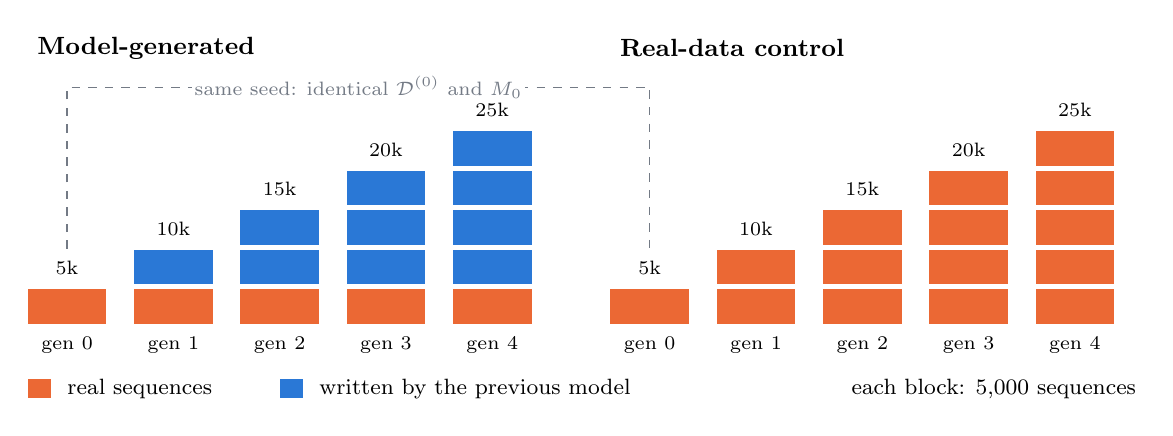
\begin{tikzpicture}
\fill[realorange] (0.00,0.00) rectangle (1.00,0.44);
\node[font=\scriptsize, above] at (0.50,0.50) {5k};
\node[font=\scriptsize, below] at (0.50,-0.05) {gen 0};
\fill[realorange] (1.35,0.00) rectangle (2.35,0.44);
\fill[modelblue] (1.35,0.50) rectangle (2.35,0.94);
\node[font=\scriptsize, above] at (1.85,1.00) {10k};
\node[font=\scriptsize, below] at (1.85,-0.05) {gen 1};
\fill[realorange] (2.70,0.00) rectangle (3.70,0.44);
\fill[modelblue] (2.70,0.50) rectangle (3.70,0.94);
\fill[modelblue] (2.70,1.00) rectangle (3.70,1.44);
\node[font=\scriptsize, above] at (3.20,1.50) {15k};
\node[font=\scriptsize, below] at (3.20,-0.05) {gen 2};
\fill[realorange] (4.05,0.00) rectangle (5.05,0.44);
\fill[modelblue] (4.05,0.50) rectangle (5.05,0.94);
\fill[modelblue] (4.05,1.00) rectangle (5.05,1.44);
\fill[modelblue] (4.05,1.50) rectangle (5.05,1.94);
\node[font=\scriptsize, above] at (4.55,2.00) {20k};
\node[font=\scriptsize, below] at (4.55,-0.05) {gen 3};
\fill[realorange] (5.40,0.00) rectangle (6.40,0.44);
\fill[modelblue] (5.40,0.50) rectangle (6.40,0.94);
\fill[modelblue] (5.40,1.00) rectangle (6.40,1.44);
\fill[modelblue] (5.40,1.50) rectangle (6.40,1.94);
\fill[modelblue] (5.40,2.00) rectangle (6.40,2.44);
\node[font=\scriptsize, above] at (5.90,2.50) {25k};
\node[font=\scriptsize, below] at (5.90,-0.05) {gen 4};
\fill[realorange] (7.40,0.00) rectangle (8.40,0.44);
\node[font=\scriptsize, above] at (7.90,0.50) {5k};
\node[font=\scriptsize, below] at (7.90,-0.05) {gen 0};
\fill[realorange] (8.75,0.00) rectangle (9.75,0.44);
\fill[realorange] (8.75,0.50) rectangle (9.75,0.94);
\node[font=\scriptsize, above] at (9.25,1.00) {10k};
\node[font=\scriptsize, below] at (9.25,-0.05) {gen 1};
\fill[realorange] (10.10,0.00) rectangle (11.10,0.44);
\fill[realorange] (10.10,0.50) rectangle (11.10,0.94);
\fill[realorange] (10.10,1.00) rectangle (11.10,1.44);
\node[font=\scriptsize, above] at (10.60,1.50) {15k};
\node[font=\scriptsize, below] at (10.60,-0.05) {gen 2};
\fill[realorange] (11.45,0.00) rectangle (12.45,0.44);
\fill[realorange] (11.45,0.50) rectangle (12.45,0.94);
\fill[realorange] (11.45,1.00) rectangle (12.45,1.44);
\fill[realorange] (11.45,1.50) rectangle (12.45,1.94);
\node[font=\scriptsize, above] at (11.95,2.00) {20k};
\node[font=\scriptsize, below] at (11.95,-0.05) {gen 3};
\fill[realorange] (12.80,0.00) rectangle (13.80,0.44);
\fill[realorange] (12.80,0.50) rectangle (13.80,0.94);
\fill[realorange] (12.80,1.00) rectangle (13.80,1.44);
\fill[realorange] (12.80,1.50) rectangle (13.80,1.94);
\fill[realorange] (12.80,2.00) rectangle (13.80,2.44);
\node[font=\scriptsize, above] at (13.30,2.50) {25k};
\node[font=\scriptsize, below] at (13.30,-0.05) {gen 4};
\node[font=\small\bfseries, anchor=west] at (0,3.5) {Model-generated};
\node[font=\small\bfseries, anchor=west] at (7.4,3.5) {Real-data control};
\draw[inkmuted, dashed] (0.5,0.95) -- (0.5,3.0) -- (7.9,3.0) -- (7.9,0.95);
\node[font=\scriptsize, text=inkmuted, fill=white, inner sep=1pt] at (4.2,3.0) {same seed: identical $\data{0}$ and $M_0$};
\fill[realorange] (0,-0.95) rectangle (0.3,-0.7);
\node[font=\footnotesize, anchor=west] at (0.38,-0.83) {real sequences};
\fill[modelblue] (3.2,-0.95) rectangle (3.5,-0.7);
\node[font=\footnotesize, anchor=west] at (3.58,-0.83) {written by the previous model};
\node[font=\footnotesize, anchor=east] at (14.2,-0.83) {each block: 5{,}000 sequences};
\end{tikzpicture}
\caption{Training-pool composition by generation. Both pools grow by 5{,}000
sequences per generation, so anything the two runs share is the effect of more
data; only the gap between them is the effect of training on model output.}
\label{fig:pool}
\end{figure}

\subsection{Revision 4: replicate across seeds}
\paragraph{Problem.} The most interesting signal of the first run, the
model's probability on symbols outside the context rising from 2.0\% to 4.5\%,
came from a single seed. One run cannot separate an effect from that run's
luck.
\paragraph{Change.} \code{-{}-seeds} runs independent replicates, each into
its own directories, and \code{src/plot\_extended\_comparison.py} draws every
seed alongside the mean. This report uses seeds 1, 2 and 3 in each condition.

\subsection{Smaller corrections}
\begin{itemize}[leftmargin=1.4em]
  \item \textbf{One model per point.} The original summary figure put $M_i$'s
        test accuracy next to statistics of $\data{i}$, which $M_{i-1}$ wrote,
        so two different models shared each generation. Single-run figures
        now use only $M_i$'s own test metrics.
  \item \textbf{The right accuracy baseline.} Accuracy plots show the 0.60
        no-binding baseline next to chance at 0.20.
  \item \textbf{Behavioural, not mechanistic.} Self-consistency had been
        called a mechanistic probe; it is a behavioural one.
\end{itemize}

\begin{table}[htbp]
\centering
\footnotesize
\setlength{\tabcolsep}{4pt}
\caption{The first full run, before the revisions (seed 5, trained to the last
step, no control). Histogram columns describe $\data{i}$ (written by
$M_{i-1}$); the last three columns are $M_i$'s own next-symbol distribution on
the test set (full-vocabulary entropy, unrenormalised preferred-symbol
probability, probability outside the context).}
\label{tab:firstrun}
\begin{tabular}{crccccccccc}
\toprule
 & & \multicolumn{3}{c}{Test accuracy / consistency} & \multicolumn{2}{c}{Histogram of $\data{i}$} & \multicolumn{3}{c}{$M_i$'s next-symbol distribution}\\
\cmidrule(lr){3-5}\cmidrule(lr){6-7}\cmidrule(lr){8-10}
Gen & Pool & $\yq$ & $\ynext$ & Self-cons. & Entropy & Coverage & Entropy & Preferred & Off-context\\
\midrule
0 & 5{,}000 & 0.991 & 0.982 & 0.983 & 3.909 & 50 & 0.337 & 0.878 & 2.0\% \\
1 & 10{,}000 & 0.992 & 0.986 & 0.985 & 3.900 & 50 & 0.503 & 0.822 & 3.0\% \\
2 & 15{,}000 & 0.990 & 0.992 & 0.982 & 3.901 & 50 & 0.630 & 0.777 & 3.9\% \\
3 & 20{,}000 & 0.995 & 0.993 & 0.980 & 3.897 & 50 & 0.663 & 0.770 & 4.0\% \\
4 & 25{,}000 & 0.997 & 0.989 & 0.972 & 3.899 & 50 & 0.712 & 0.757 & 4.5\% \\
\bottomrule
\end{tabular}
\end{table}

% =====================================================================
\section{Experimental setup}\label{sec:setup}

\begin{table}[htbp]
\centering
\small
\caption{Configuration (\code{config\_collapse.yaml} for the base pipeline,
\code{config\_extended\_collapse.yaml} for the extended one).}
\label{tab:config}
\begin{tabular}{lll}
\toprule
Setting & Base & Extended\\
\midrule
Symbols $N$, labels $L$, context pairs $K$ & 50, 5, 2 & 50, 5, 2\\
Layers, heads, width & 2, 8, 64 & 2, 8, 64\\
Optimiser, learning rate, batch size & Adam, $10^{-4}$, 32 & Adam, $10^{-4}$, 32\\
Training steps per generation & 20{,}000 & 20{,}000\\
Evaluation interval & 500 steps & 500 steps\\
Generations & 5 (0 to 4) & 5 (0 to 4)\\
New sequences per generation & 5{,}000 & 5{,}000\\
Validation and test sets & 2{,}000 each, fixed & 2{,}000 each, fixed\\
Decoding of generated tokens & argmax & sampling, temperature 1\\
Held-out share for checkpoint selection & none & 10\%\\
\bottomrule
\end{tabular}
\end{table}

\paragraph{Conditions.} Three conditions, each with seeds 1, 2 and 3:
\begin{itemize}[leftmargin=1.4em]
  \item \textbf{Extended, model-generated}: the extended pipeline with sampled
        continuations.
  \item \textbf{Extended, real-data control}: identical, but every
        generation's continuations come from the true distribution
        (\code{-{}-control}).
  \item \textbf{Base}: the base pipeline, unchanged (argmax targets, last-step
        checkpoint, no control).
\end{itemize}
A seed fixes the data, the initialisation, the minibatch order and the
sampled continuations, so the fixed validation and test sets also differ
between seeds; each seed is an independent replicate.

\paragraph{Compute.} All runs used a laptop CPU (Intel Core i7-1255U, 10 cores)
with one thread per run, several runs in parallel. The six extended runs took
28 minutes of wall-clock time together; the three base runs took
14 minutes.

\paragraph{Reproduction.} From the repository root:
\begin{Verbatim}[fontsize=\scriptsize, frame=single, framesep=2mm]
python src/train_extended_collapse.py --config config_extended_collapse.yaml --seeds 1 2 3
python src/train_extended_collapse.py --config config_extended_collapse.yaml --control --seeds 1 2 3
python src/plot_extended_comparison.py "results/extended_collapse_metrics*_test_summary.csv"
python src/train_collapse.py --config config_collapse.yaml
\end{Verbatim}
The base script takes its seed and output paths from the configuration file;
the base runs in this report used copies of \code{config\_collapse.yaml} with
\code{seed} set to 1, 2 and 3 and seed-specific output paths.

% =====================================================================
\section{Results}\label{sec:results}

\subsection{Sanity checks}
\paragraph{Pairing.} Within each seed, the model-generated and control runs
produced identical generation-0 results, to every logged digit, in all three
seeds, as the paired design requires.

\paragraph{Checkpoint selection.} Table~\ref{tab:selection} lists the step
that selection kept. In generation 0 it stopped at step 5{,}500 in every seed,
close to where the pre-revision run's held-out loss bottomed out
(Figure~\ref{fig:overfit}). Later generations, with larger pools, stopped
later.

\begin{table}[htbp]
\centering
\small
\caption{Training step of the kept checkpoint, model-generated / control.}
\label{tab:selection}
\begin{tabular}{cccccc}
\toprule
Seed & Gen 0 & Gen 1 & Gen 2 & Gen 3 & Gen 4\\
\midrule
1 & 5{,}500 / 5{,}500 & 10{,}500 / 15{,}000 & 12{,}000 / 12{,}500 & 11{,}000 / 12{,}000 & 17{,}500 / 17{,}000 \\
2 & 5{,}500 / 5{,}500 & 8{,}000 / 7{,}500 & 17{,}500 / 11{,}000 & 17{,}000 / 12{,}000 & 17{,}000 / 16{,}000 \\
3 & 5{,}500 / 5{,}500 & 8{,}500 / 6{,}500 & 10{,}000 / 14{,}000 & 14{,}500 / 16{,}500 & 18{,}500 / 15{,}500 \\
\bottomrule
\end{tabular}
\end{table}

\subsection{Model-generated against real data}
Figure~\ref{fig:comparison} shows every seed of both conditions, and
Tables~\ref{tab:cmpA} and~\ref{tab:cmpB} give the means. Generation 0 is
shared. From generation 1 onwards the control improves on every measure as
real data accumulates, while the model-generated chain barely moves.

\begin{figure}[htbp]
\centering
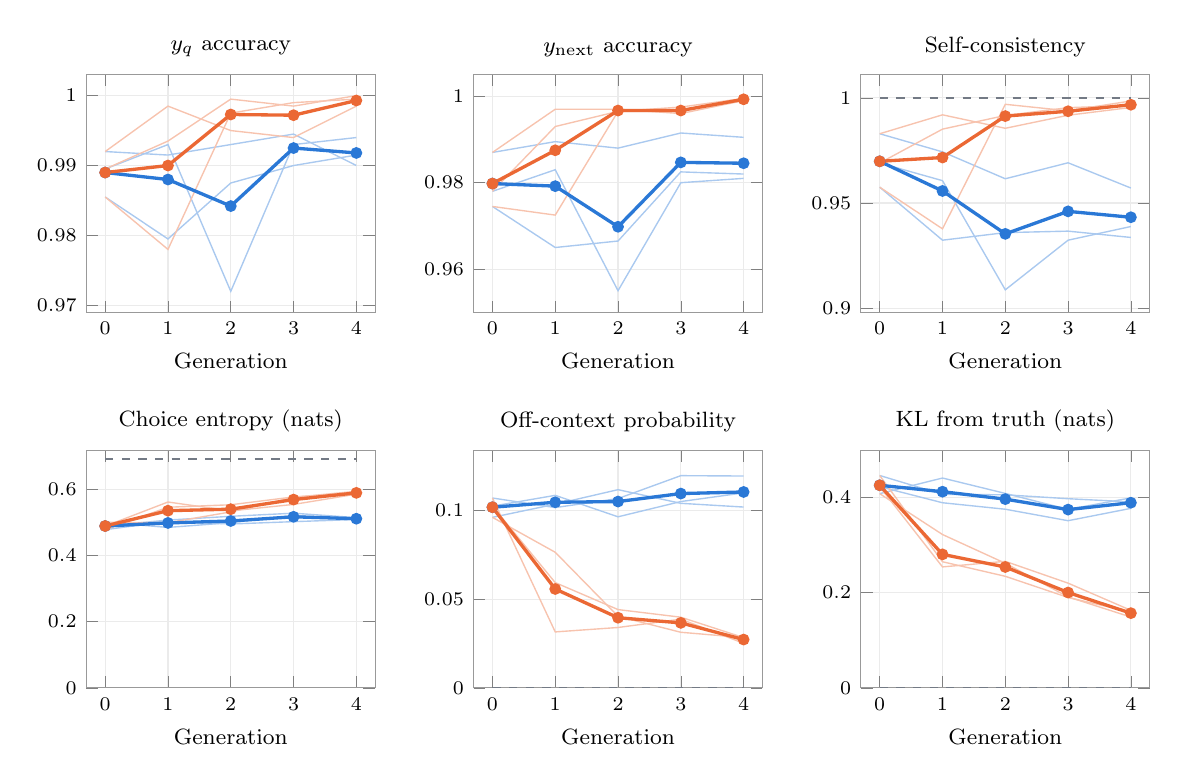
\begin{tikzpicture}
\begin{groupplot}[
  group style={group size=3 by 2, horizontal sep=1.25cm, vertical sep=1.75cm},
  collapse,
]
\nextgroupplot[title={$y_q$ accuracy}, ymin=0.969, ymax=1.003, legend to name=cmplegend, legend columns=2, legend style={/tikz/every even column/.append style={column sep=12pt}}]
\addplot[seed model] coordinates {(0,0.9855) (1,0.9795) (2,0.9875) (3,0.9900) (4,0.9915)};
\addplot[seed model] coordinates {(0,0.9895) (1,0.9930) (2,0.9720) (3,0.9930) (4,0.9940)};
\addplot[seed model] coordinates {(0,0.9920) (1,0.9915) (2,0.9930) (3,0.9945) (4,0.9900)};
\addplot[seed real] coordinates {(0,0.9855) (1,0.9780) (2,0.9975) (3,0.9990) (4,0.9995)};
\addplot[seed real] coordinates {(0,0.9895) (1,0.9935) (2,0.9995) (3,0.9985) (4,1.0000)};
\addplot[seed real] coordinates {(0,0.9920) (1,0.9985) (2,0.9950) (3,0.9940) (4,0.9985)};
\addplot[mean model] coordinates {(0,0.9890) (1,0.9880) (2,0.9842) (3,0.9925) (4,0.9918)};
\addlegendentry{Model-generated}
\addplot[mean real] coordinates {(0,0.9890) (1,0.9900) (2,0.9973) (3,0.9972) (4,0.9993)};
\addlegendentry{Real-data control}
\nextgroupplot[title={$y_{\text{next}}$ accuracy}, ymin=0.950, ymax=1.005]
\addplot[seed model] coordinates {(0,0.9745) (1,0.9650) (2,0.9665) (3,0.9825) (4,0.9820)};
\addplot[seed model] coordinates {(0,0.9780) (1,0.9830) (2,0.9550) (3,0.9800) (4,0.9810)};
\addplot[seed model] coordinates {(0,0.9870) (1,0.9895) (2,0.9880) (3,0.9915) (4,0.9905)};
\addplot[seed real] coordinates {(0,0.9745) (1,0.9725) (2,0.9965) (3,0.9965) (4,0.9995)};
\addplot[seed real] coordinates {(0,0.9780) (1,0.9930) (2,0.9965) (3,0.9975) (4,0.9995)};
\addplot[seed real] coordinates {(0,0.9870) (1,0.9970) (2,0.9970) (3,0.9960) (4,0.9990)};
\addplot[mean model] coordinates {(0,0.9798) (1,0.9792) (2,0.9698) (3,0.9847) (4,0.9845)};
\addplot[mean real] coordinates {(0,0.9798) (1,0.9875) (2,0.9967) (3,0.9967) (4,0.9993)};
\nextgroupplot[title={Self-consistency}, ymin=0.898, ymax=1.011]
\addplot[ref line, domain=0:4, samples=2] {1.0000};
\addplot[seed model] coordinates {(0,0.9575) (1,0.9323) (2,0.9359) (3,0.9366) (4,0.9336)};
\addplot[seed model] coordinates {(0,0.9690) (1,0.9606) (2,0.9087) (3,0.9323) (4,0.9388)};
\addplot[seed model] coordinates {(0,0.9829) (1,0.9743) (2,0.9615) (3,0.9691) (4,0.9571)};
\addplot[seed real] coordinates {(0,0.9575) (1,0.9377) (2,0.9969) (3,0.9938) (4,0.9985)};
\addplot[seed real] coordinates {(0,0.9690) (1,0.9851) (2,0.9916) (3,0.9953) (4,0.9964)};
\addplot[seed real] coordinates {(0,0.9829) (1,0.9919) (2,0.9855) (3,0.9917) (4,0.9954)};
\addplot[mean model] coordinates {(0,0.9698) (1,0.9557) (2,0.9353) (3,0.9460) (4,0.9432)};
\addplot[mean real] coordinates {(0,0.9698) (1,0.9716) (2,0.9913) (3,0.9936) (4,0.9967)};
\nextgroupplot[title={Choice entropy (nats)}, ymin=0.000, ymax=0.719]
\addplot[ref line, domain=0:4, samples=2] {0.6931};
\addplot[seed model] coordinates {(0,0.5009) (1,0.4851) (2,0.4996) (3,0.5212) (4,0.5105)};
\addplot[seed model] coordinates {(0,0.4783) (1,0.5035) (2,0.4955) (3,0.5026) (4,0.5091)};
\addplot[seed model] coordinates {(0,0.4890) (1,0.5074) (2,0.5188) (3,0.5282) (4,0.5147)};
\addplot[seed real] coordinates {(0,0.5009) (1,0.4993) (2,0.5321) (3,0.5762) (4,0.5945)};
\addplot[seed real] coordinates {(0,0.4783) (1,0.5462) (2,0.5537) (3,0.5774) (4,0.5889)};
\addplot[seed real] coordinates {(0,0.4890) (1,0.5620) (2,0.5352) (3,0.5547) (4,0.5858)};
\addplot[mean model] coordinates {(0,0.4894) (1,0.4987) (2,0.5046) (3,0.5173) (4,0.5115)};
\addplot[mean real] coordinates {(0,0.4894) (1,0.5358) (2,0.5403) (3,0.5694) (4,0.5897)};
\nextgroupplot[title={Off-context probability}, ymin=0.000, ymax=0.134]
\addplot[ref line, domain=0:4, samples=2] {0.0000};
\addplot[seed model] coordinates {(0,0.1070) (1,0.1016) (2,0.1067) (3,0.1196) (4,0.1194)};
\addplot[seed model] coordinates {(0,0.1024) (1,0.1085) (2,0.0964) (3,0.1050) (4,0.1099)};
\addplot[seed model] coordinates {(0,0.0961) (1,0.1035) (2,0.1117) (3,0.1040) (4,0.1019)};
\addplot[seed real] coordinates {(0,0.1070) (1,0.0315) (2,0.0340) (3,0.0387) (4,0.0251)};
\addplot[seed real] coordinates {(0,0.1024) (1,0.0593) (2,0.0441) (3,0.0398) (4,0.0283)};
\addplot[seed real] coordinates {(0,0.0961) (1,0.0764) (2,0.0403) (3,0.0313) (4,0.0283)};
\addplot[mean model] coordinates {(0,0.1018) (1,0.1046) (2,0.1050) (3,0.1095) (4,0.1104)};
\addplot[mean real] coordinates {(0,0.1018) (1,0.0557) (2,0.0395) (3,0.0366) (4,0.0272)};
\nextgroupplot[title={KL from truth (nats)}, ymin=0.000, ymax=0.499]
\addplot[ref line, domain=0:4, samples=2] {0.0000};
\addplot[seed model] coordinates {(0,0.4076) (1,0.4404) (2,0.4081) (3,0.3746) (4,0.3987)};
\addplot[seed model] coordinates {(0,0.4457) (1,0.4061) (2,0.4052) (3,0.3970) (4,0.3903)};
\addplot[seed model] coordinates {(0,0.4223) (1,0.3885) (2,0.3749) (3,0.3508) (4,0.3767)};
\addplot[seed real] coordinates {(0,0.4076) (1,0.3218) (2,0.2614) (3,0.1908) (4,0.1485)};
\addplot[seed real] coordinates {(0,0.4457) (1,0.2646) (2,0.2341) (3,0.1896) (4,0.1590)};
\addplot[seed real] coordinates {(0,0.4223) (1,0.2538) (2,0.2655) (3,0.2197) (4,0.1626)};
\addplot[mean model] coordinates {(0,0.4252) (1,0.4117) (2,0.3961) (3,0.3741) (4,0.3886)};
\addplot[mean real] coordinates {(0,0.4252) (1,0.2801) (2,0.2536) (3,0.2000) (4,0.1567)};
\end{groupplot}
\end{tikzpicture}

\smallskip
\pgfplotslegendfromname{cmplegend}
\caption{Extended pipeline, model-generated data (blue) against the matched
real-data control (orange). Thin lines are individual seeds, thick lines the
mean over the three seeds. Dashed lines are analytic reference values
(Table~\ref{tab:reference}); in the two accuracy panels the no-binding
baseline of 0.60 lies below the plotted range.}
\label{fig:comparison}
\end{figure}

\begin{table}[htbp]
\centering
\small
\caption{Accuracy and self-consistency on the fixed test set, mean over three
seeds (model-generated / control).}
\label{tab:cmpA}
\begin{tabular}{c*{3}{cc}}
\toprule
 & \multicolumn{2}{c}{$\yq$ accuracy} & \multicolumn{2}{c}{$\ynext$ accuracy} & \multicolumn{2}{c}{Self-consistency}\\
\cmidrule(lr){2-3}\cmidrule(lr){4-5}\cmidrule(lr){6-7}
Gen & Model & Control & Model & Control & Model & Control\\
\midrule
0 & 0.989 & 0.989 & 0.980 & 0.980 & 0.970 & 0.970 \\
1 & 0.988 & 0.990 & 0.979 & 0.987 & 0.956 & 0.972 \\
2 & 0.984 & 0.997 & 0.970 & 0.997 & 0.935 & 0.991 \\
3 & 0.992 & 0.997 & 0.985 & 0.997 & 0.946 & 0.994 \\
4 & 0.992 & 0.999 & 0.984 & 0.999 & 0.943 & 0.997 \\
\bottomrule
\end{tabular}
\end{table}

\begin{table}[htbp]
\centering
\small
\setlength{\tabcolsep}{4.5pt}
\caption{Next-symbol metrics on the fixed test set, mean over three seeds
(model-generated / control). Truth: entropy 0.693, preferred 0.5, off-context
0, KL 0.}
\label{tab:cmpB}
\begin{tabular}{c*{4}{cc}}
\toprule
 & \multicolumn{2}{c}{Choice entropy} & \multicolumn{2}{c}{Preferred prob.} & \multicolumn{2}{c}{Off-context prob.} & \multicolumn{2}{c}{KL from truth}\\
\cmidrule(lr){2-3}\cmidrule(lr){4-5}\cmidrule(lr){6-7}\cmidrule(lr){8-9}
Gen & Model & Control & Model & Control & Model & Control & Model & Control\\
\midrule
0 & 0.489 & 0.489 & 0.760 & 0.760 & 0.102 & 0.102 & 0.425 & 0.425 \\
1 & 0.499 & 0.536 & 0.753 & 0.727 & 0.105 & 0.056 & 0.412 & 0.280 \\
2 & 0.505 & 0.540 & 0.750 & 0.723 & 0.105 & 0.039 & 0.396 & 0.254 \\
3 & 0.517 & 0.569 & 0.741 & 0.700 & 0.110 & 0.037 & 0.374 & 0.200 \\
4 & 0.511 & 0.590 & 0.745 & 0.682 & 0.110 & 0.027 & 0.389 & 0.157 \\
\bottomrule
\end{tabular}
\end{table}

\subsection{Paired differences}
Table~\ref{tab:gaps} gives the paired gap (model-generated minus control)
at generation 4. In every metric the three seeds agree in sign, and the gap is
between 2.7 and 12.9 times its seed-to-seed standard deviation.
Table~\ref{tab:gapgen} shows that the gap grows with the generation for the
next-symbol metrics, again with all three seeds agreeing in sign in every
generation.

\begin{table}[htbp]
\centering
\small
\setlength{\tabcolsep}{4pt}
\caption{Paired gap at generation 4, model-generated minus control, over three
seeds. ``Gap/s.d.'' is the mean gap over the standard deviation of the three
per-seed gaps. $p$ is a two-sided paired $t$-test with 2 degrees of freedom;
with three seeds such tests are fragile, and the consistency across seeds and
generations is the stronger evidence.}
\label{tab:gaps}
\begin{tabular}{lcccccc}
\toprule
Metric & Model & Control & Mean gap & Range over seeds & Gap/s.d. & $p$\\
\midrule
KL from truth (nats) & 0.389 & 0.157 & $+0.232$ & $+0.214$ to $+0.250$ & 12.9 & 0.002 \\
Off-context probability & 0.110 & 0.027 & $+0.083$ & $+0.074$ to $+0.094$ & 8.0 & 0.005 \\
Choice entropy (nats) & 0.511 & 0.590 & $-0.078$ & $-0.084$ to $-0.071$ & 11.9 & 0.002 \\
Preferred-symbol probability & 0.745 & 0.682 & $+0.063$ & $+0.055$ to $+0.070$ & 8.2 & 0.005 \\
Self-consistency & 0.943 & 0.997 & $-0.054$ & $-0.065$ to $-0.038$ & 3.9 & 0.021 \\
$y_{\text{next}}$ accuracy & 0.984 & 0.999 & $-0.015$ & $-0.018$ to $-0.009$ & 2.7 & 0.043 \\
$y_q$ accuracy & 0.992 & 0.999 & $-0.007$ & $-0.008$ to $-0.006$ & 5.7 & 0.010 \\
\bottomrule
\end{tabular}
\end{table}

\begin{table}[htbp]
\centering
\small
\caption{Mean paired gap (model-generated minus control) by generation. In
every cell the three seeds agree in sign.}
\label{tab:gapgen}
\begin{tabular}{ccccc}
\toprule
Gen & KL from truth & Off-context prob. & Choice entropy & Self-consistency\\
\midrule
1 & $+0.132$ & $+0.049$ & $-0.037$ & $-0.016$ \\
2 & $+0.142$ & $+0.065$ & $-0.036$ & $-0.056$ \\
3 & $+0.174$ & $+0.073$ & $-0.052$ & $-0.048$ \\
4 & $+0.232$ & $+0.083$ & $-0.078$ & $-0.054$ \\
\bottomrule
\end{tabular}
\end{table}

\subsection{What the model-generated data contains}
Table~\ref{tab:data} describes the training data each model wrote. $M_0$ put
about 10\% of its next-symbol probability outside the context, so about 10\%
of the next symbols in $\data{1}$ were symbols that never appeared in the
sequence. The share then crept upwards as each model learned from data that
already contained such errors.

\begin{table}[htbp]
\centering
\small
\caption{Generated data in the model-generated condition, three seeds: the
share of sequences whose next symbol is outside the context (mean and range),
the agreement of the generated $\yq$ with the truth, and the data's
self-consistency. Row $i$ describes $\data{i}$, written by $M_{i-1}$; row 0 is
real data.}
\label{tab:data}
\begin{tabular}{ccccc}
\toprule
$\data{i}$ & Outside context & Range & $\yq$ agreement & Self-consistency\\
\midrule
0 & 0.0\% & 0.0--0.0\% & 1.000 & 1.000 \\
1 & 10.0\% & 9.2--10.6\% & 0.975 & 0.968 \\
2 & 10.7\% & 10.1--11.6\% & 0.967 & 0.961 \\
3 & 10.9\% & 10.5--11.2\% & 0.955 & 0.935 \\
4 & 11.6\% & 10.6--13.1\% & 0.966 & 0.950 \\
\bottomrule
\end{tabular}
\end{table}

\subsection{The view without a control}
Table~\ref{tab:chain} compares the model-generated chain with itself and with
the control. Read on its own, the chain looks stable: KL from the truth even
falls slightly, and the off-context probability rises by under one percentage
point. That reading would conclude ``no collapse''. The control shows what the
same growth in data does when the data is real: KL falls to 0.157 and leakage
to 2.7\%. The model-generated chain does not stay still so much as fail to
improve, while its leakage and self-consistency drift slowly the wrong way.

\begin{table}[htbp]
\centering
\small
\caption{The model-generated chain against itself and against the control
(means over three seeds).}
\label{tab:chain}
\begin{tabular}{lccc}
\toprule
Metric & Model-generated, gen 0 & Model-generated, gen 4 & Control, gen 4\\
\midrule
KL from truth (nats) & 0.425 & 0.389 & 0.157 \\
Off-context probability & 0.102 & 0.110 & 0.027 \\
Choice entropy (nats) & 0.489 & 0.511 & 0.590 \\
Self-consistency & 0.970 & 0.943 & 0.997 \\
\bottomrule
\end{tabular}
\end{table}

\subsection{Base pipeline}
Table~\ref{tab:base} and Figure~\ref{fig:base} give the base pipeline's
results over the same three seeds. Test accuracy starts at 0.997 in generation 0 and ends at 0.999 in generation 4, and the targets each model wrote for the next generation agree with the truth in 99.72\% to 99.96\% of sequences. The base pipeline shows no sign of collapse. With at most 0.28\% of its labels wrong, model-written data is almost indistinguishable from real data, and accuracy rises slightly as the pool grows, as it would with real data. Without a matched control the base pipeline cannot separate those two explanations, but with labels this accurate the distinction hardly matters. The base model is also slightly more accurate than the extended model's $\yq$ in either condition; the extended model learns three tokens and is stopped earlier by checkpoint selection, so that difference reflects the training setup, not recursion.

\begin{table}[htbp]
\centering
\small
\caption{Base pipeline, three seeds, with the extended pipeline's
query-label results for comparison. Agreement in row $i$ refers to the targets
of $\data{i}$, written by $M_{i-1}$ (row 0 is real data).}
\label{tab:base}
\begin{tabular}{ccccccc}
\toprule
 & \multicolumn{4}{c}{Base} & \multicolumn{2}{c}{Extended, model-generated}\\
\cmidrule(lr){2-5}\cmidrule(lr){6-7}
Gen & Test acc. & Range & Test loss & Label agreement & $\yq$ test acc. & $\yq$ agreement\\
\midrule
0 & 0.9973 & 0.9965--0.9980 & 0.0087 & 1.0000 & 0.9890 & 1.0000 \\
1 & 0.9988 & 0.9985--0.9990 & 0.0043 & 0.9983 & 0.9880 & 0.9748 \\
2 & 0.9985 & 0.9975--0.9995 & 0.0055 & 0.9992 & 0.9842 & 0.9671 \\
3 & 0.9988 & 0.9985--0.9995 & 0.0055 & 0.9990 & 0.9925 & 0.9554 \\
4 & 0.9993 & 0.9985--1.0000 & 0.0036 & 0.9995 & 0.9918 & 0.9659 \\
\bottomrule
\end{tabular}
\end{table}

\begin{figure}[htbp]
\centering
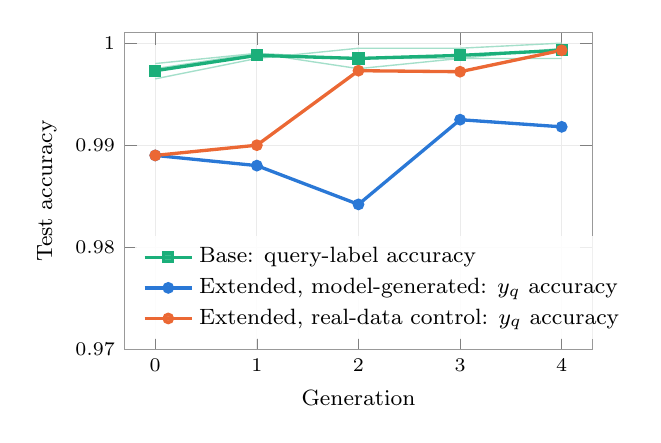
\begin{tikzpicture}
\begin{axis}[
  collapse, width=0.62\linewidth, height=5.6cm,
  ymin=0.97, ymax=1.001, ylabel={Test accuracy}, ylabel style={font=\footnotesize},
  legend style={at={(0.02,0.03)}, anchor=south west, fill=white, fill opacity=0.85, text opacity=1},
]
\addplot[seed base] coordinates {(0,0.9965) (1,0.9985) (2,0.9995) (3,0.9995) (4,1.0000)};
\addplot[seed base] coordinates {(0,0.9975) (1,0.9990) (2,0.9975) (3,0.9985) (4,0.9985)};
\addplot[seed base] coordinates {(0,0.9980) (1,0.9990) (2,0.9985) (3,0.9985) (4,0.9995)};
\addplot[mean base] coordinates {(0,0.9973) (1,0.9988) (2,0.9985) (3,0.9988) (4,0.9993)};
\addlegendentry{Base: query-label accuracy}
\addplot[mean model] coordinates {(0,0.9890) (1,0.9880) (2,0.9842) (3,0.9925) (4,0.9918)};
\addlegendentry{Extended, model-generated: $y_q$ accuracy}
\addplot[mean real] coordinates {(0,0.9890) (1,0.9900) (2,0.9973) (3,0.9972) (4,0.9993)};
\addlegendentry{Extended, real-data control: $y_q$ accuracy}
\end{axis}
\end{tikzpicture}
\caption{Query-label accuracy across generations: base pipeline (green; thin
lines are seeds) and the extended pipeline's $\yq$ in both conditions
(means over three seeds).}
\label{fig:base}
\end{figure}

% =====================================================================
\section{Discussion}\label{sec:discussion}

\subsection{What the results show}
Training on model output did not make the extended model collapse in the
runaway sense: accuracy stayed above 0.97 and no metric deteriorated sharply.
What it did was \emph{lock in} the first model's errors. $M_0$, stopped at the
best held-out loss, leaked about 10\% of its next-symbol probability outside
the context and was overconfident in its choice between the two context
symbols (0.76 on its favourite, where the truth is 0.5). Sampling from $M_0$
wrote those errors into $\data{1}$, and every later model learned them as part
of the task. The real-data control, given the same growth in data, unlearned
them: by generation 4 its leakage fell to 2.7\% and its KL from the truth to
0.157 nats, against 11.0\% and 0.389 nats in the model-generated chain.

This matches the accumulate regime of Gerstgrasser et
al.~\cite{gerstgrasser2024}: because $\data{0}$ stays in the pool, real data
anchors every generation and the error stays bounded. Yet the anchor's weight
shrinks from 100\% of the pool to 20\% by generation 4, and the gap to the
control widens each generation, so the model-generated chain is not standing
still relative to what the same amount of real data would achieve.

\subsection{Mechanism}
Two channels carry the errors forward. First, \emph{leakage}: off-context
symbols in the generated data teach the next model that the next symbol is
sometimes not in the context at all, so its own leakage persists and slowly
grows (10.0\% of $\data{1}$ to 11.6\% of $\data{4}$). Second,
\emph{overconfidence}: $M_0$'s preferences between the two context symbols are
a function of the context, so they are learnable. Sampled continuations
encode those preferences as if they were real structure, and the next model
imitates them, which keeps its choice entropy near 0.5 nats while the
control's rises towards $\log 2$. Self-consistency falls because the
generated data contains $\ynext$ labels that do not match their $\xnext$
(Table~\ref{tab:data}), weakening the symbol-to-label binding the third token
depends on.

\subsection{Base against extended}
The base task has one deterministic output, so recursive training can only
corrupt it through wrong labels, and its model makes almost none.
Its model-written labels were wrong in at most 0.28\% of sequences in any generation, so recursive training had almost nothing to propagate, and accuracy rose slightly, from 0.997 to 0.999, as the pool grew. The extended task exposes what accuracy cannot: its
deterministic tokens stay at or above 0.97 accuracy in both conditions, but the
distribution over the stochastic token, the leakage and the binding on the
model's own outputs all separate the model-generated chain from the control.
A collapse study that only measured accuracy would have reported no effect in
either pipeline.

\subsection{The role of checkpoint selection}
Selection changed which errors $M_0$ passes on. Trained to the last step
(first run), $M_0$ was strongly overconfident (choice entropy 0.337) but leaked
little (2.0\%); stopped at the best held-out loss, it is less overconfident
(0.489) but leaks more (10.2\%). The magnitude of every effect in this report
therefore depends on $M_0$'s error profile. A better $M_0$, trained on more
real data or with regularisation, would pass on fewer errors. The direction of
the effect, model-generated data preserving errors that real data removes,
does not depend on this choice.

\subsection{Limitations}
\begin{itemize}[leftmargin=1.4em]
  \item \textbf{Three seeds.} Every seed agrees in sign, but formal tests with
        three replicates are fragile.
  \item \textbf{Accumulation only.} The pool keeps all real data, which
        damps collapse by design. A replace regime would test the stronger
        form of collapse.
  \item \textbf{No rare-event tail.} The true next-symbol distribution is a
        fair coin, so the classic signature of collapse, rare outcomes
        disappearing~\cite{shumailov2024}, cannot occur in this task.
  \item \textbf{The base pipeline is not matched.} It keeps the last-step
        checkpoint and has no control, so base and extended differ in those
        respects as well as in the task.
  \item \textbf{One decoding rule and one task size.} Only sampling at
        temperature 1 and $K=2$ were run.
  \item \textbf{Behavioural evidence.} No result here identifies an
        induction circuit or shows how it changes across generations.
\end{itemize}

\subsection{Future work}
\begin{itemize}[leftmargin=1.4em]
  \item Run the replace regime alongside accumulation.
  \item Make the next-symbol distribution skewed (more context symbols with
        unequal probabilities) so that rare-but-valid continuations exist and
        their disappearance can be measured.
  \item Give the base pipeline the same checkpoint selection and control.
  \item Run the \code{argmax} and \code{hybrid} decoding contrasts.
  \item Track attention patterns and head ablations across generations to
        connect the behavioural effects to the induction circuit.
\end{itemize}

% =====================================================================
\section{Conclusion}
In a fully controlled in-context learning task, recursive training on
model-generated data did not produce runaway collapse, as expected when real
data accumulates. It did preserve the first model's errors, leakage outside
the context, overconfident choices and weaker binding, which real data of the
same quantity removed, and the gap widened every generation in all three
seeds. Seeing this required measuring the next-symbol distribution through the
model's own probabilities, stopping $M_0$ before it memorised its pool, and
comparing against a matched real-data control. Without those, the same
experiment would have reported ``no collapse'', for reasons that had nothing to
do with the model.

% =====================================================================
\appendix
\section{Repository map}
\begin{center}
\small
\begin{tabularx}{\linewidth}{lX}
\toprule
File & Purpose\\
\midrule
\code{src/data.py}, \code{src/model.py} & base task generator and the attention-only transformer\\
\code{src/collapse\_data.py}, \code{src/train\_collapse.py} & base recursive pipeline\\
\code{src/extended\_data.py} & extended three-token task\\
\code{src/extended\_model.py} & extended readout on the shared blocks\\
\code{src/extended\_collapse\_data.py} & autoregressive rollout and data generation\\
\code{src/extended\_metrics.py} & collapse metrics, including \code{next\_symbol\_stats}\\
\code{src/train\_extended\_collapse.py} & extended pipeline: selection, \code{-{}-control}, \code{-{}-seeds}\\
\code{src/plot\_extended\_collapse\_metrics.py} & figures for one run\\
\code{src/plot\_extended\_comparison.py} & comparison figure across conditions and seeds\\
\code{results/*\_test\_summary.csv} & per-generation summaries, one per run\\
\code{results/extended\_comparison.png} & comparison figure (PNG version of Figure~\ref{fig:comparison})\\
\bottomrule
\end{tabularx}
\end{center}

\section{Summary CSV columns (extended pipeline)}
\begin{center}
\small
\begin{tabularx}{\linewidth}{lX}
\toprule
Column & Meaning\\
\midrule
\code{seed}, \code{continuation\_source}, \code{decode} & run identity (\code{model} or \code{real}; decoding rule)\\
\code{selected\_step} & training step of the kept checkpoint\\
\code{test\_loss\_t1..t3}, \code{test\_acc\_t1..t3} & per-token loss and accuracy of $M_i$ on the fixed test set\\
\code{test\_next\_context\_entropy} & choice entropy $\bar H$\\
\code{test\_next\_preferred\_prob} & preferred-symbol probability $\bar\pi$\\
\code{test\_next\_off\_context\_mass} & off-context probability $\bar o$\\
\code{test\_next\_kl\_to\_truth} & KL from the truth\\
\code{test\_consistency}, \code{test\_type\_validity} & self-consistency and type validity of $M_i$'s own rollouts\\
\code{data\_*} & statistics of $\data{i}$, written by $M_{i-1}$ (row 0: real data)\\
\code{data\_in\_context\_fraction} & share of $\data{i}$ whose $\xnext$ is a context symbol\\
\code{data\_symbol\_*} & emitted-symbol histogram (global bias check only)\\
\bottomrule
\end{tabularx}
\end{center}

% =====================================================================
\begin{thebibliography}{9}
\bibitem{shumailov2024}
I.~Shumailov, Z.~Shumaylov, Y.~Zhao, N.~Papernot, R.~Anderson and Y.~Gal.
\newblock AI models collapse when trained on recursively generated data.
\newblock \emph{Nature}, 631:755--759, 2024.

\bibitem{gerstgrasser2024}
M.~Gerstgrasser, R.~Schaeffer, A.~Dey, et al.
\newblock Is model collapse inevitable? Breaking the curse of recursion by
accumulating real and synthetic data.
\newblock arXiv:2404.01413, 2024.

\bibitem{olsson2022}
C.~Olsson, N.~Elhage, N.~Nanda, et al.
\newblock In-context learning and induction heads.
\newblock \emph{Transformer Circuits Thread}, 2022.

\bibitem{singh2024}
A.~K.~Singh, T.~Moskovitz, F.~Hill, S.~C.~Y.~Chan and A.~M.~Saxe.
\newblock What needs to go right for an induction head? A mechanistic study of
in-context learning circuits and their formation.
\newblock In \emph{Proceedings of the 41st International Conference on Machine
Learning (ICML)}, 2024.

\bibitem{su2021}
J.~Su, Y.~Lu, S.~Pan, A.~Murtadha, B.~Wen and Y.~Liu.
\newblock RoFormer: Enhanced transformer with rotary position embedding.
\newblock arXiv:2104.09864, 2021.

\bibitem{kingma2015}
D.~P.~Kingma and J.~Ba.
\newblock Adam: A method for stochastic optimization.
\newblock In \emph{International Conference on Learning Representations
(ICLR)}, 2015.
\end{thebibliography}

\end{document}
